\begin{exr}
Què passa segons l'Equació de van der Waals si la pressió es fa propera a zero o bé la temperatura es fa molt gran per a un gas real?   La figura mostra el factor de compressibilitat per a un mateix gas a diferents temperatures
\begin{center}        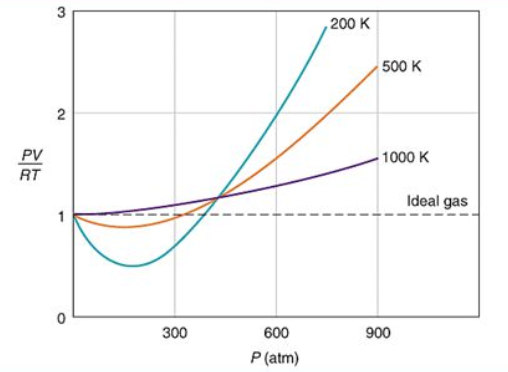
\includegraphics[scale=1.0]{FactorCompressT.png}
\end{center}
\end{exr}